\section{Casting QoE Optimization as a Exploration-Exploitation Process}
\label{sec:pytheas:casting}

To avoid these aforementioned limitations of prediction-based approaches, ideally we
want a framework  where decisions are updated in concert with measurement collection in real time.
%decisions and measurements are made in concert and
%updated in real time. 
%This could ideally  avoid unnecessary measurement collection, overloading decisions \vyas{vague},
% and adapt to flashcrowd swiftly.  
There is indeed a well-known abstraction in the
machine learning community that captures this---\mablong (\mab) 
processes~\cite{mab}.  Drawing on this parallel, we argue why   data-driven QoE
optimization should be cast instead as a {\em real-time \mab} process rather
than a prediction-based workflow.
%We begin by providing some brief background on \mab.
% 
% before showing how we cast  data-driven QoE optimization as 
% an \mab process (Figure~\ref{fig:casting}). 

%In contrast to the prediction-oriented abstraction% which predicts quality periodically by separately collected measurements (Figure~\ref{fig:abstraction-intro}(a)), 
%we take a first-principles approach and argue that the abstraction for data-driven quality optimization should be a {\em real-time \mablong (\mab)} process, where decisions and measurements are made in concert and updated in real time. 


%We use \mablong (or \mab), borrowed from machine learning literature, as a systematic formulation for \ddn problem. 
%\vyas{u need to do more handholding here -- what are teh two EEs etc}
\mypara{Background on \mablong} An intuitive way to visualize the \mablong (\mab) process is through the lens of 
a  multi-armed bandit problem~\cite{mab}.  Here, a gambler pulls
several slot machines, each associated with 
an unknown reward distribution.
The goal of the gambler is to optimize
the mean rewards over a sequence of pulls. 
 Thus, there is some intrinsic {\em exploration} phase where
 the gambler tries to learn these hidden reward functions, and subsequent  
{\em exploitation} phase to maximize the reward. Note that the reward 
 functions could  change over time, and thus this is a 
 continuous process rather than a one-time shot.
 
\mypara{QoE optimization as \mab (Figure~\ref{fig:casting})}  Given this framework,  we can see a natural mapping between \mab and data-driven QoE optimization.  
Like \mab, data-driven QoE optimization observes the QoE (i.e., reward) of a decision
every time the decision is used (i.e., pulled) by a session.
  Our goal is to maximize the overall QoE after a sequence of 
sessions.
%In \mab, each
%slot machine is associate with a reward distribution, an equivalent of each
%decision having some QoE distribution in data-driven QoE optimization.
%Moreover, both problems share the goal of optimizing overall rewards (QoE)
%within a limited number of pulls (or sessions).

Casting data-driven optimization as \mab not only provides 
a systematic framework for data-driven QoE optimization, 
but also allows us to leverage well-known algorithms (e.g.,~\cite{ucb1}) from the  machine learning literature.  
As \mab integrates the measurement collection (exploration) and 
decision making (exploitation) in a joint process,
we can dynamically explore decisions whose 
quality estimation has high uncertainty, and exploit decisions
that are clearly better.  For instance, in Example A, an \mab process could
 reduce traffic for exploration when QoE is stable (before 40
second and after 120 seconds), and raise it when QoE changes
(between 40 second and 120 second).  By running \mab in real time with the
most up-to-date measurement data, we could detect QoE drift as soon as some
sessions have experienced them, and adapt to them faster than
prediction-based approaches.  For instance, in Example B, real-time \mab
would detect load-induced QoE degradation on CDN1 as soon as its QoE is
worse than CDN2, and start switching sessions to CDN2 {\em before} overloading
CDN1.\footnote{Note that we do not need to know the capacity of each CDN, which is often unknown to content providers.}  
%Real-time
%\mab can also be robust to flash crowd. For instance, in Example C, if we
%detect the flash crowd as soon as it happens, we could separate sessions of the
%flash crowd and customize their decisions without affecting others.


 
%For instance, application quality vary over time, and to
%optimize quality under such time-varying distributions, we can borrow \mab
%techniques designed for non-stationary bandits (see more details in
%\Section\ref{subsec:??}).




\begin{figure}[t!]
\centering
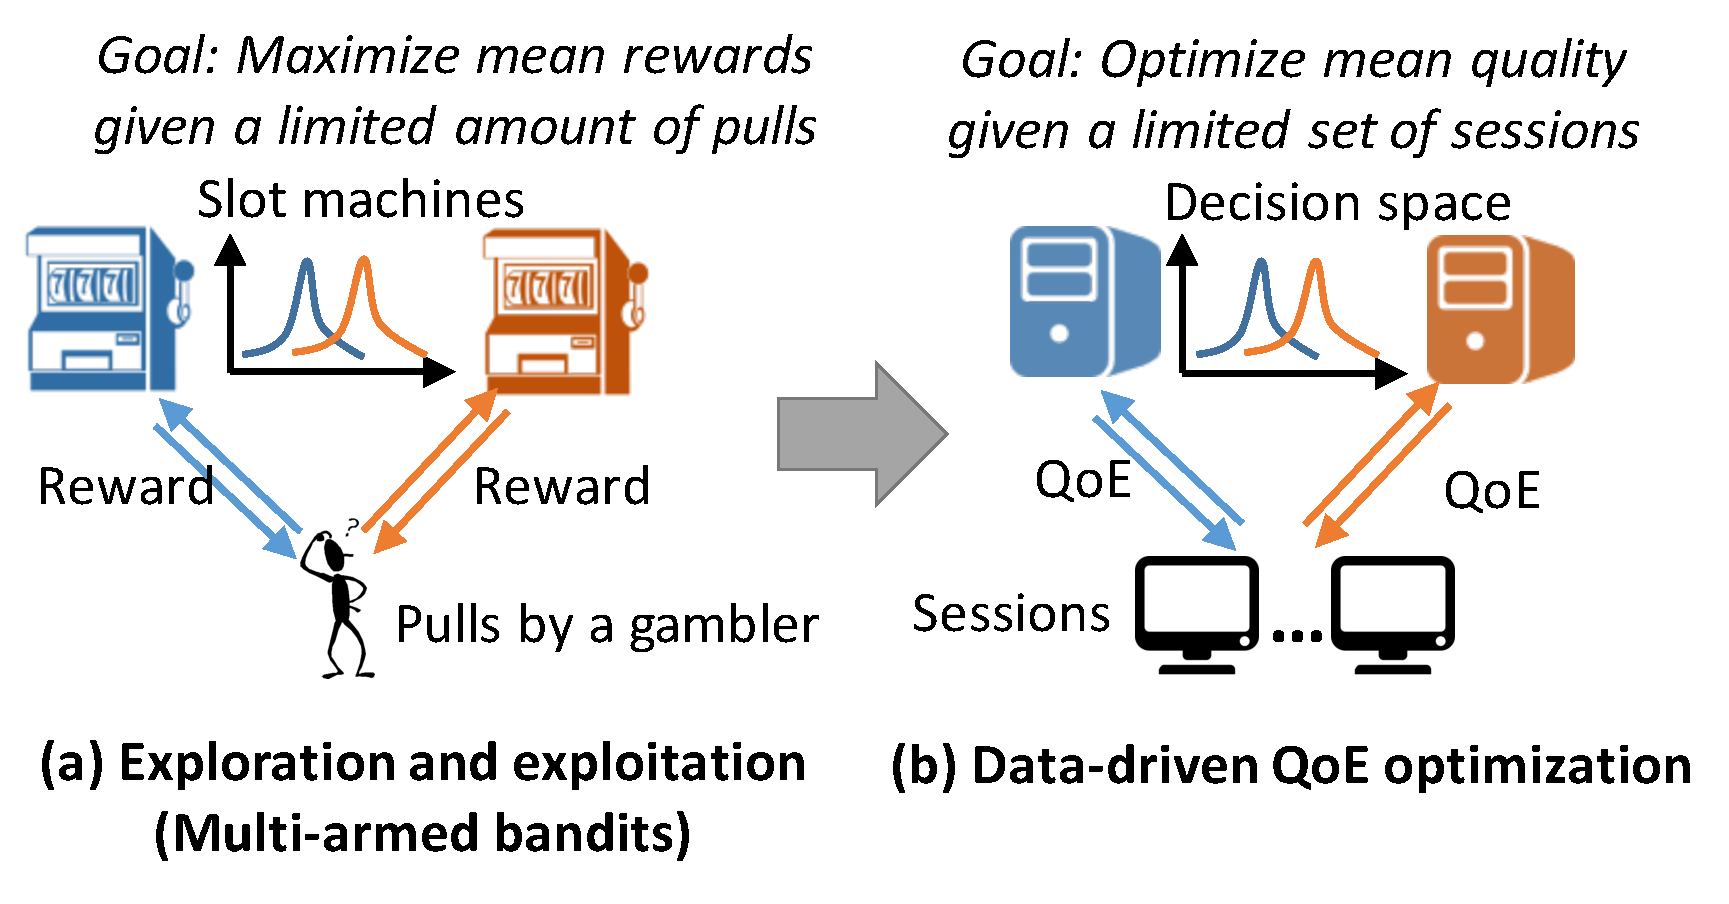
\includegraphics[width=0.7\textwidth]{figures/pytheas-casting.pdf}
%\vspace{-0.5cm}
\caption{Casting data-driven QoE optimization into formulation of \mablong (\mab).}
\label{fig:casting}
\end{figure}

\subsection{Challenges of E2 in the Networking Context}
While \mab offers the right abstraction in contrast to prediction-based approaches,
 applying it in network applications raises practical challenges:
\begin{packeditemize}
\item %{\em How to run real-time \mab over millions of globally distributed sessions with fresh data?} \\ 
%Running \mab at scale with real-time feedback is challenging, because 
Traditional \mab
techniques (e.g.,~\cite{mab,linucb,velox-cidr}) need fresh measurements of all sessions, 
but getting such a fresh and global view is challenging, because application providers
store fresh data in geo-distributed clusters, called {\em frontend clusters}, which only have a partial view across sessions.
Existing analytics framework for such geo-distributed infrastructure, however, either trade global view for
data freshness (e.g.,~\cite{c3}), or target query patterns of a traditional database (e.g.,~\cite{iris}), not
millions of concurrent queries from geo-distributed clients, as in our case.

%Unfortunately, many seemingly
%natural strawman solutions do not address this challenge.  For instance, split
%control architecture~\cite{c3} makes decisions by frontend clusters based on
%fresh data of the same session and stale data on other sessions.  It is
%reasonable to trade data freshness for scalability and responsiveness, when
%best decisions do not change often, but when quality or request pattern
%suddenly changes, split control will fall back to local adaptation, when
%multi-session view is needed the most to maintain desirable quality.
%Similarly, distributed data analytics platforms   store in geo-distributed
%clusters, but their existing solutions are not suitable for \ddn.  One approach
%assumes that data can be efficiently centralized in lower fidelity~\cite{??},
%but it is unclear how to reduce fidelity of quality measurements without
%letting \mab make suboptimal decisions.  Another approach performs analytics
%jobs in a distributed way and aggregates results in real time~\cite{??}, which
%is suitable to handle tens of requests per second, but it is not desirable to
%update \mab decisions for millions of sessions. \vyas{too much text and noise.
%please shrink}



%To guarantee responsiveness to globally distributed
%clients, application providers have deployed geo-distributed frontend
%clusters~\cite{??,??}, so that the user activities and logs (including quality
%measurements) are first stored in frontend clusters and periodically archived
%to a backend on coarse timescale of minutes or hours~\cite{c3} and often in
%lower fidelity~\cite{jetstream}.  Therefore, neither frontend nor backend
%provides a fresh and global view of measurements needed by \mab algorithms.

%First, we need to a system architecture that updates the \mab decision in real time with the most up-to-date measurement data, and responds to client requests very quickly.
%This is challenging, because \mab techniques (e.g.,~\cite{linucb,velox}) need fresh and global view of measurement data, whereas service providers store fresh client data in geo-distributed clusters, each having only a partial view.
%To serve globally distributed clients, application providers today have deployed geo-distributed frontend clusters~\cite{??,??} so that the
%user activities and logs (including quality measurement) are first stored one of clusters and periodically updated to a backend on coarse timescale of minutes or hours and often in lower fidelity. 
%This makes it difficult to maintain a fresh view of all data to update MAB decision, as it takes time to gather the sheer size of measurement data from different frontend clusters to where decisions are made. 
%Such situation would even be common, if contextual MAB algorithm (e.g.,~\cite{linucb,velox}) needs a global view of measurement data to make decisions.
%For instance, even though MAB techniques can react fast enough in theory where decision is updated with the most recent feedback, their reaction speed would be bottlenecked by the existence of substantial feedback delay.


%\vspace{0.1cm}\noindent{\bf How to model networking ``context'' in MAB?}
\item %{\em How to model ``network context'' in \mab?}\\
Traditional \mab techniques also make strong assumptions about the context
that affects the reward of a decisions, but they may not hold in network settings.
For instance, they often assume some notion of
continuity in context (e.g.,~\cite{cmab}), but even when some video sessions match on
all aspects of ISP, location, CDN resource availability, they 
may still see very different QoE, if they differ on certain key feature 
(e.g., last-hop connection)~\cite{cfa}.

%Network sessions with different network contexts (e.g., last-mile connections, WAN performance,
%CDN resource availability, and device information) should not be treated identical in an \mab process.
%One option is to use so called ``contextual multi-armed
%bandit''~\cite{cmab} techniques, where rewards of a
%bandit also depends on the context of a certain pull, but they often assume some notion of
%continuity in context, but two network sessions that match on all features
%except one can still have very different network performance~\cite{cfa}.

%Application sessions with different network ``contexts'' do not share same
%optimal decisions, so \mab process should be aware of the network context,
%rather than treating all sessions identically.  For instance, video quality
%depends on complex factors including last-mile connections, WAN performance,
%CDN resource availability, and device information, and sometimes, their
%combinations~\cite{cfa}, so the degree to which one session's quality should
%affect the selection of CDNs, bitrate, or network path of another session
%varies greatly across sessions.  One option is to use ``contextual multi-armed
%bandit''~\cite{??} techniques from \mab literature, which assumes rewards of a
%bandit depends on the context of a pull, but they often assume some notion of
%continuity in context; e.g., similar contexts always yield similar
%rewards~\cite{??}, whereas two network sessions that match on all features
%except one can still have very different network performance~\cite{cfa}.
%Alternatively, we can use more domain-specific techniques
%(e.g.,~\cite{cfa,cs2p}), but they are designed for quality prediction.  For
%instance, CFA uses critical features to mode sessions with similar quality, but
%critical features do not indicate whether a session should explore different
%decisions to optimize the quality for future sessions.
% \vyas{too much text and noise.
%please shrink - not more than 5-6 lines for each challenge}



\end{packeditemize}


%For instance, CFA only predicts for each session which decision should be exploited under contextual settings, but it does not decide when it should be used to explore different decisions.

%CMAB techniques, however, are no panacea, especially in a networking context. 

%\begin{packedenumerate}
%\item Need for context: quality distributions differ across sessions.
%\item Contextual MAB requires domain-specific modeling of the context.
%\end{packedenumerate}



%\begin{packedenumerate}
%\item MAB cannot react fast (even though it logically can), if the feedback delay is on timescale of minutes.
%\item It's challenging for existing architecture to achieve required feedback delay for MAB.
%\end{packedenumerate}










